% contributors: Alper Cakan
\section{Embedding Delauney Graphs Into Hyperbolic Planes}

Now we discuss \cite{Sarkar}. 
In this paper, the authors study the embeddings of Delauney graphs into hyperbolic planes. 
The above notes should serve as a good background for the hyperbolic setting that will be considered henceforth.
Delaunay graphs have quite useful properties and are well studied. 
Therefore finding an embedding of a graph such that the resulting set's Delaunay graph is the same as the original graph would allow us to use these properties and the results from the related literature. This paper focuses on embedding trees into the hyperbolic plane with low distortion and with this property, that the Delaunay graph of the embedded points gives the original tree back.
\subsection{Preliminaries}
\subsubsection{Delaunay Graphs}
Let's start by some equivalent definitions of the Delaunay graphs.
\begin{definition}
A Delaunay triangulation of a set of points S is a triangulation such that no point of S is inside the circumcircle of any of the triangles of the triangulation. The graph of a Delaunay triangulation is called a Delaunay graph.
\end{definition}

Although this is the usual definition, the paper provides an equivalent one that is more useful for our purposes:

\begin{definition}
A set of vertices in the hyperbolic plane is called a Delaunay graph if vertex pairs are connected if and only if their Voronoi cells intersect.
\end{definition}

\subsubsection{Cones in the Hyperbolic Plane}
An important tool in the construction will be so-called cones in the hyperbolic plane.

\begin{definition}
Two parallel lines are called limiting parallel or critically parallel if they never \textit{touch} but they get arbitrarily close asymptotically.
\end{definition}

As a simplification, to have an image, think of $y = \frac{1}{x}$ and $y = -\frac{1}{x}$ in the Euclidean plane.

\begin{definition}
Two parallel lines are called divergent parallel or ultraparallel if they have a closest point and they diverge from each other.
\end{definition}

Again, to have a picture in your mind, think of an hyperbola (whose center axis is parallel to x-axis) and its mirror image w.r.t y-axis in the usual Euclidean plane.

It's a simple property that for any point and a line not passing through it, there is some point on the line such that the \textit{segment} from that to the other point is perpendicular to the line. (This part is also true for Euclidean space). Yet another simple yet crucial property is that we can draw a pair of diverging parallel lines from that outside point such that:

\begin{itemize}
    \item They have symmetric angles with the segment
    \item They are limiting parallel the original line in both directions
\end{itemize}

Figure \ref{fig:cone} shows all of these in action. The region bounded by the original line and the constructed limiting line pair is called a \textit{closed cone}. Note that the position of the original line and the outside point, or equivalently the outside point and the symmetric angles determine cone uniquely. We can create arbitrarily (but finitely) many cones whose apex is the same fixed point by taking different rays, which induce different segments, and we can make all these cones disjoint by picking the rays so that the symmetric angles are small enough.

\begin{figure}
    \centering
    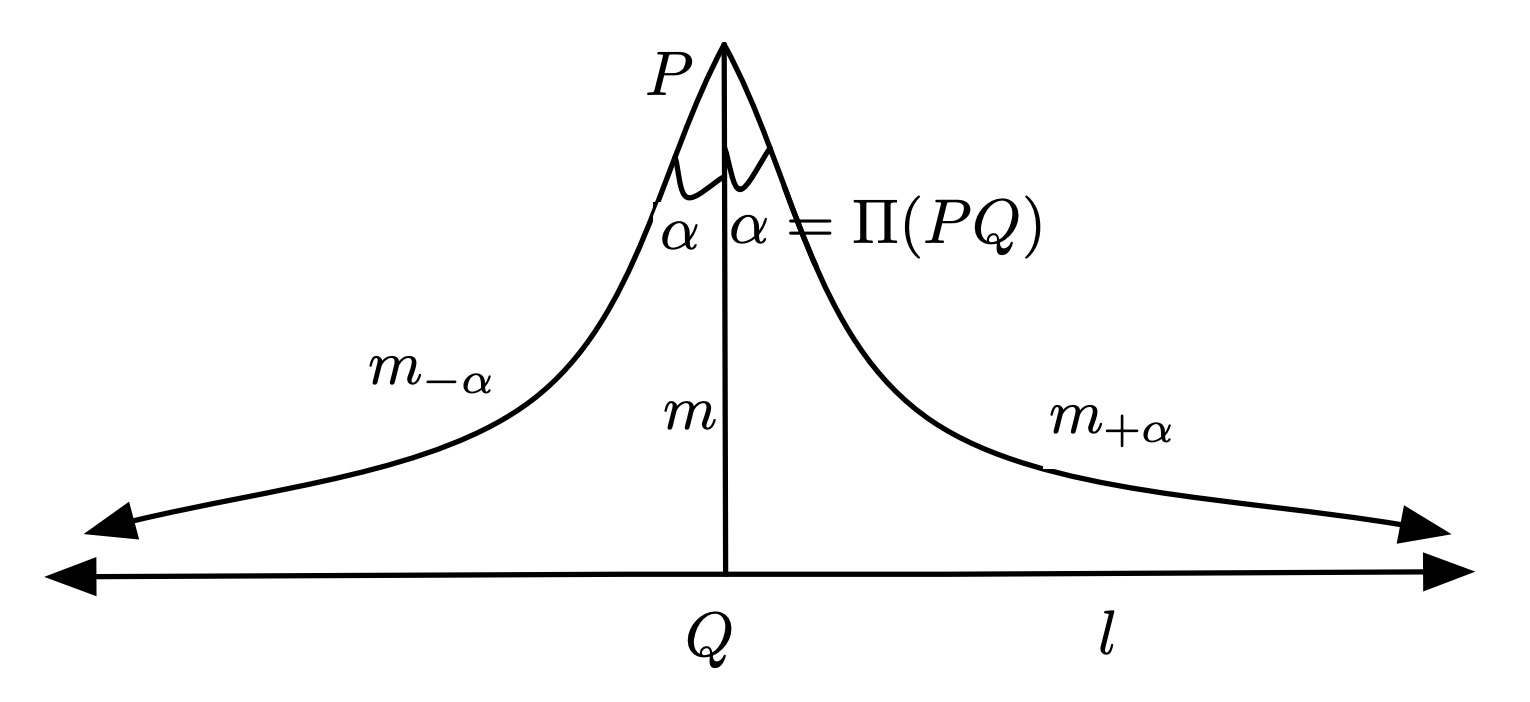
\includegraphics[width=.7\textwidth]{chapter_14/files/cone.png}
    \caption{Closed Cone}
    \label{fig:cone}
\end{figure}

\subsection{Delaunay Embeddings of Trees}
First, we will construct an algorithm to embed unweighted trees as Delaunay graphs. We will then gradually build on this embed metric trees \footnote{Weighted tree with shortest path metric} as Delaunay graphs with low distortion.

Consider any vertex as the root to make the tree into a rooted tree. The algorithm is as follows: \\
\rule{\linewidth}{0.5pt} \\
1. Map the root $v_0$ to any point, say $p_0$. \\
2. Delaunay-embed $d$ children of the root into $d$ disjoint cones whose apex are at $p_0$. \\
3. Continue embedding recursively as follows: if $v_i$ is a child of $v_j$, embed children of $v_i$ in disjoint cones that are also disjoint from the $v_i$ $v_j$ embedding cone.  \\
\rule{\linewidth}{0.5pt} \\

\begin{figure}
    \centering
    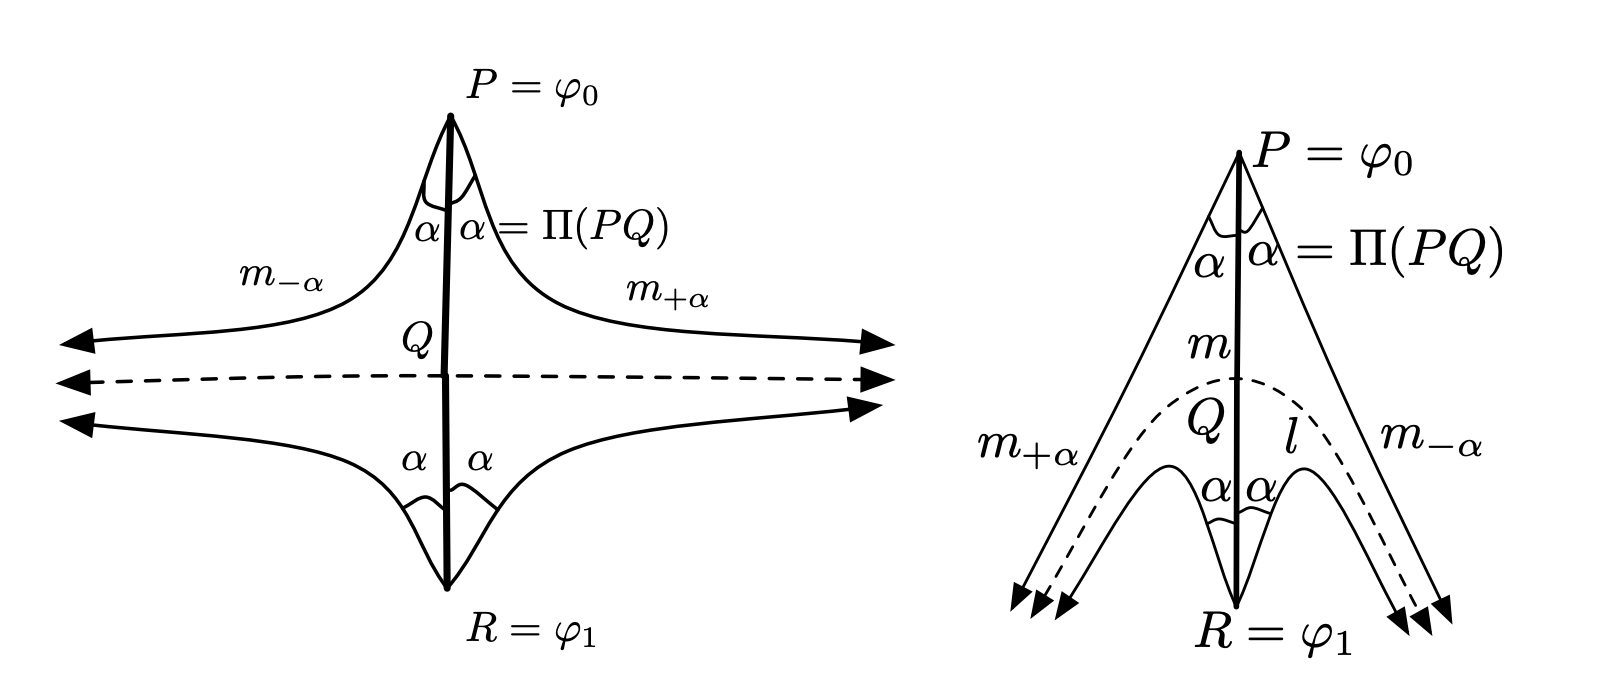
\includegraphics[width=\textwidth]{chapter_14/files/cone2.png}
    \caption{Embedding of a vertex (at P) and its child (at R), representations from the \textit{points of views} of child and parent respectively}
    \label{fig:cone_two}
\end{figure}

\begin{figure}
    \centering
    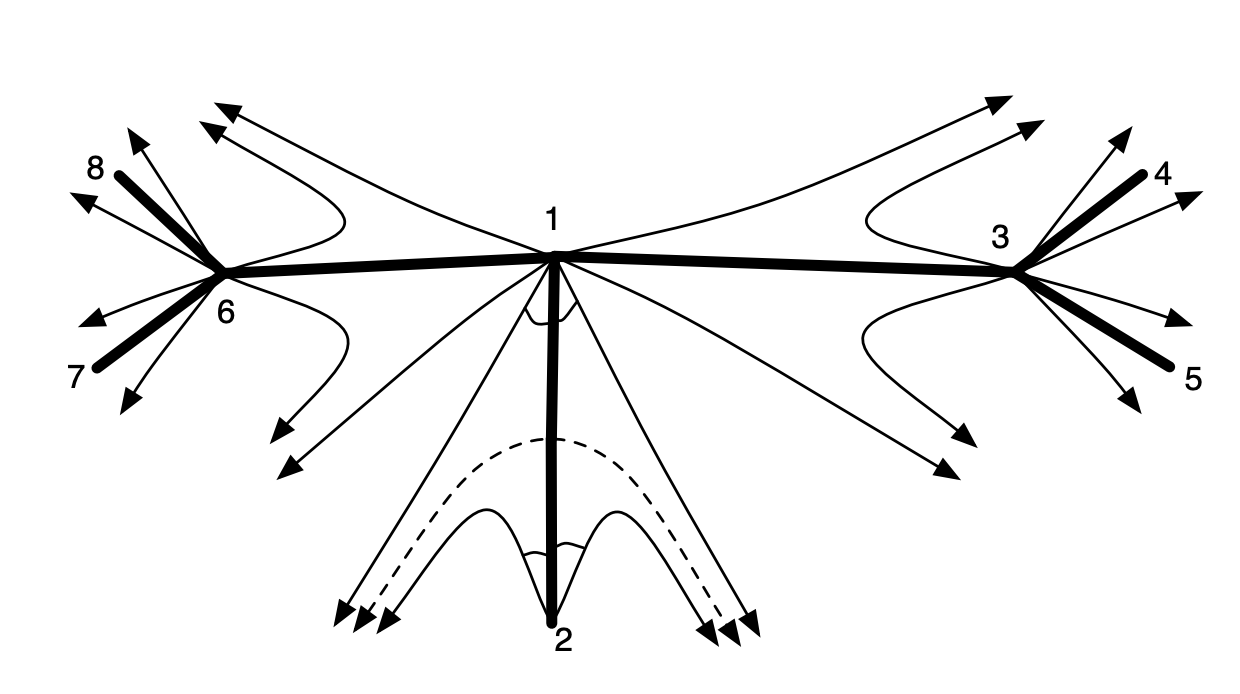
\includegraphics[width=\textwidth]{chapter_14/files/conem.png}
    \caption{Cone-based representation of the embedding of a whole tree}
    \label{fig:cone_multiple}
\end{figure}

Notice that we assumed we can \textit{Delaunay-embed} individual edges. Here is how we can do it. We choose angles $\alpha$ small enough to ensure disjointness, and for a given edge (one vertex already fixed, say as $p_0$) and its $\alpha$, pick a $p_1$ such that $$|p_0p_1|_{\mathbb{H}} \geq -2k\ln(tan(\frac{\alpha}{2}))$$ See Figures \ref{fig:cone_two} and \ref{fig:cone_multiple} for a visualization.

\subsection{Delaunay Embeddings of Metric Trees}
Based on the previous embedding, we can actually obtain a stronger one. This time we are considering weighted trees. We want the resulting embedding to capture the \textit{geometry} of the tree, that is, we want the distances of the embedded points to be the same as the weight of the corresponding edge in the original tree (up to a constant that is the same for all edges). We can in fact achieve this, but note that this not the same as embedding a metric tree isometrically: the shortest path distances between vertices that are not adjacent will not stay the same after the embedding. We will denote edge weight between $u$ and $v$ as $w_{u,v}$

The embedding algorithm is quite similar to the unweighted case, and is as follows. For each edge $v_0, v_1$ where $v_0$ is the direct parent of $v_1$,: \\
\rule{\linewidth}{0.5pt} \\
1. Create $degree(v_1) - 1$ cones (whose apex are at embedding of $v_1$) that are disjoint from the $v_0v_1$ embedding cone and also pairwise disjoint (by picking small enough angles). \\
2. Embed children of $v_1$ as follows: Any child $v_2$ is embedded with a cone as before such that $v_1$, $v_2$ distance in the hyperbolic plane is $\eta \cdot w_{v_1, v_2}$  \\
\rule{\linewidth}{0.5pt} \\

Observe that this is the same as the algorithm before, except that we specify the embedding distance more carefully. But again, we embed a child-parent pair as in Figure \ref{fig:cone_two}.

Lastly, we made use of a constant $\eta$. This is a constant which is picked as the maximum of required scaling factors over all edges in the tree. That is, for each edge, there is a minimum scaled factor needed so that the embedded edge is a Delaunay edge. We calculate this number for all edges, and take the maximum over all edges and apply the same scale to all edges so that: (i) all edges are embedded as Delaunay edges, (ii) all edges are scaled by the same amount.

\subsection{Reducing the Distortion}
As we mentioned above, the embedding we have so far can only guarantee that each edge length will scale by the same factor. However, the distance between vertices that are not adjacent will not scale the same way, since the tree metric can only follow the edges whereas the hyperbolic plane metric is not bound by the edges.

However, it turns out that we can use a similar algorithm that can give an embedding with $1 + \epsilon$ distortion for any $\epsilon > 0$. Note that this involves a trade-off, and see the next section for more details.

\begin{definition}
Two cones that share an apex are $\beta$-separated if they're $2\beta$ angles apart.
\end{definition}

Now, the main theorem that helps us build an embedding with arbitrarily low distortion.

\begin{theorem}
If the following are all true an embedding of a tree, then its distortion is bounded by $1 + \epsilon$
\begin{itemize}
    \item is Delaunay,
    \item all cone pairs used by the embedding are $\beta$-separated for some suitably small constant $\beta$,
    \item all edges are scaled by the same factor $\tau > \eta$ such that each edge becomes longer than $\nu\frac{1+\epsilon}{\epsilon}$, where $\nu$ is a constant that only depends on $\beta$.
\end{itemize}
\end{theorem}

Using this theorem, the following algorithm gives the desired embedding: \\
\rule{\linewidth}{0.5pt} \\
1. Compute the constant $\nu$ and the cone angle $\alpha$ as follows: Find small enough $\beta$ ($< \frac{\pi}{d_{max}}$, where $d_{max}$ is the highest degree in tree), then $\nu = -2k\ln(\tan(\frac{\beta}{2}))$ and $\alpha = \frac{2\pi}{d_{max}} - 2\beta$.
2. Compute $\eta$ as before. \\
3. Compute $\tau$ such that all edges become longer than $\nu\frac{1+\epsilon}{\epsilon}$.
4. Use the embedding algorithm from the previous section, but scale by  $\tau$ instead of $\eta$ and enforce $\beta$-separated cones.\\
\rule{\linewidth}{0.5pt} \\